\clearpage
%% ============================================================
\section{Pełny loss LeJEPA}
\label{sec:fulloss}
%% ============================================================

\begin{equation}
\boxed{
\mathcal{L}_{\text{LeJEPA}} =
\underbrace{\frac{\lambda}{V} \sum_{v=1}^{V} \mathrm{SIGReg}\!\left(\{\mathbf{z}_{n,v}\}_{n=1}^B\right)}_{\text{regularyzacja: wymuś } \mathcal{N}(\mathbf{0}, \mathbf{I})}
+ \underbrace{\frac{1-\lambda}{B} \sum_{n=1}^{B} \mathcal{L}_{\text{pred}}^{(V_g)}\!\left(\{\mathbf{z}_{n,v}\}_{v=1}^V\right)}_{\text{predykcja: wymuś semantyczną spójność}}
}
\label{eq:lejepa}
\end{equation}

gdzie loss predykcyjny to:
\begin{equation}
\mathcal{L}_{\text{pred}} = \frac{1}{V}\sum_{v'=1}^{V}
\left\|\boldsymbol{\mu}_n - \mathbf{z}_{n,v'}\right\|_2^2,
\quad
\boldsymbol{\mu}_n \triangleq \frac{1}{V_g}\sum_{v=1}^{V_g} \mathbf{z}_{n,v}
\label{eq:pred_loss}
\end{equation}

\begin{keyinsight}[Jeden hiperparametr!]
$\lambda$ kontroluje trade-off między:
\begin{itemize}
  \item $\lambda \to 0$: czysta predykcja (ryzyko kolapsu),
  \item $\lambda \to 1$: czysty SIGReg (brak semantycznej struktury),
  \item $\lambda = 0.05$: \textbf{rekomendowane} — stabilne na wielu datasetach i architekturach.
\end{itemize}
\end{keyinsight}

%% --- Szczegółowe wyjaśnienie wzoru (25) ---
\subsection{Jak czytać wzór (\ref{eq:lejepa}) --- słownik symboli}

Zanim przeczytamy wzór, ustalmy co oznacza \textbf{każdy symbol}:

\begin{center}
\renewcommand{\arraystretch}{1.4}
\begin{tabular}{c p{10cm}}
\toprule
\textbf{Symbol} & \textbf{Znaczenie} \\
\midrule
$\mathcal{L}_{\text{LeJEPA}}$ &
  Pełna \textbf{funkcja straty} (loss) --- jedna liczba, którą sieć minimalizuje
  w~każdym kroku treningu. Im mniejsza, tym lepiej. \\
$\lambda$ &
  \textbf{Hiperparametr balansujący} --- liczba z~przedziału $[0, 1]$
  (typowo $0{.}05$). Kontroluje proporcję:
  ile ``uwagi'' poświęcamy regularyzacji, a~ile predykcji. \\
$V$ &
  \textbf{Liczba wszystkich widoków} (views) jednego obrazu.
  W~LeJEPA: $V = V_g + V_l$, np.\ $V = 2 + 6 = 8$
  (2~globalne + 6~lokalnych). \\
$V_g$ &
  \textbf{Liczba widoków globalnych} (global views) ---
  duże kadrowania ($224 \times 224$) z~jednego obrazu. Typowo $V_g = 2$. \\
$V_l$ &
  \textbf{Liczba widoków lokalnych} (local views) ---
  małe kadrowania ($96 \times 96$). Typowo $V_l = 6$. \\
$B$ &
  \textbf{Rozmiar batcha} --- ile obrazów przetwarzamy na raz
  (np.\ $B = 256$). \\
$n$ &
  \textbf{Indeks obrazu} w~batchu: $n \in \{1, 2, \ldots, B\}$. \\
$v$ &
  \textbf{Indeks widoku}: $v \in \{1, 2, \ldots, V\}$. \\
$\mathbf{z}_{n,v} \in \mathbb{R}^d$ &
  \textbf{Embedding} $n$-tego obrazu z~$v$-tego widoku ---
  wektor $d$-wymiarowy (np.\ $d = 128$) wyprodukowany
  przez sieć (ViT + projektor). \\
$\mathrm{SIGReg}(\cdot)$ &
  Regularyzator z~sekcji~9.5 --- mierzy, jak daleko embeddingi
  są od rozkładu $\mathcal{N}(\mathbf{0}, \mathbf{I})$. \\
$\mathcal{L}_{\text{pred}}$ &
  \textbf{Loss predykcyjny} --- mierzy, jak bardzo embeddingi różnych
  widoków \textit{tego samego} obrazu różnią się od siebie. \\
$\boldsymbol{\mu}_n$ &
  \textbf{Centroid} (średnia) embeddingów widoków globalnych
  $n$-tego obrazu. Punkt odniesienia, do którego
  porównujemy wszystkie widoki. \\
$\|\cdot\|_2^2$ &
  \textbf{Kwadrat normy euklidesowej} --- suma kwadratów
  różnic po współrzędnych: $\|\mathbf{a} - \mathbf{b}\|_2^2 = \sum_i (a_i - b_i)^2$. \\
$\triangleq$ &
  ``\textbf{definiujemy jako}'' --- symbol oznacza, że lewa strona jest
  \textit{nową definicją}, nie wynikiem obliczeń. \\
\bottomrule
\end{tabular}
\end{center}

\subsection{Czytanie wzoru (\ref{eq:lejepa}) od lewej do prawej}

Teraz czytamy wzór po polsku, symbol po symbolu:

\begin{tcolorbox}[colback=blue!4, colframe=blue!60!black, breakable,
  title={\textbf{Wzór (\ref{eq:lejepa}) --- jak go przeczytać}}]

\[
\mathcal{L}_{\text{LeJEPA}} =
\underbrace{\frac{\lambda}{V} \sum_{v=1}^{V} \mathrm{SIGReg}\!\left(\{\mathbf{z}_{n,v}\}_{n=1}^B\right)}_{\text{część A}}
+
\underbrace{\frac{1-\lambda}{B} \sum_{n=1}^{B} \mathcal{L}_{\text{pred}}^{(V_g)}\!\left(\{\mathbf{z}_{n,v}\}_{v=1}^V\right)}_{\text{część B}}
\]

\textbf{Część A --- regularyzacja SIGReg:}

\medskip
Czytamy: \textit{``Weź wagę $\lambda$, podziel przez liczbę widoków $V$,
i~dla każdego widoku $v$ od 1 do $V$ policz SIGReg
na zbiorze embeddingów wszystkich $B$ obrazów w~tym widoku.''}

\begin{enumerate}[leftmargin=2em]
  \item Fiksujemy widok $v$ (np.\ ``widok globalny nr~1'').
  \item Zbieramy embeddingi \textbf{tego widoku} ze~wszystkich obrazów w~batchu:
        $\{\mathbf{z}_{1,v},\; \mathbf{z}_{2,v},\; \ldots,\; \mathbf{z}_{B,v}\}$
        --- to $B$ wektorów w~$\mathbb{R}^d$.
  \item Sprawdzamy SIGRegiem: czy te $B$ wektorów tworzą
        rozkład $\mathcal{N}(\mathbf{0}, \mathbf{I})$?
  \item Powtarzamy dla każdego widoku $v = 1, \ldots, V$ i~uśredniamy ($\div V$).
  \item Mnożymy przez wagę $\lambda$ (typowo $0{.}05$).
\end{enumerate}

\textbf{Intuicja}: regularyzacja sprawdza \textit{kolumnami} ---
``czy chmura embeddingów z~każdego widoku wygląda jak izotropowy Gauss?''

\bigskip
\textbf{Część B --- predykcja:}

\medskip
Czytamy: \textit{``Weź wagę $(1-\lambda)$, podziel przez liczbę obrazów $B$,
i~dla każdego obrazu $n$ policz loss predykcyjny na wszystkich jego widokach.''}

\begin{enumerate}[leftmargin=2em]
  \item Fiksujemy obraz $n$ (np.\ ``zdjęcie kota nr~17'').
  \item Zbieramy embeddingi \textbf{tego obrazu} ze~wszystkich widoków:
        $\{\mathbf{z}_{n,1},\; \mathbf{z}_{n,2},\; \ldots,\; \mathbf{z}_{n,V}\}$.
  \item Liczymy centroid z~widoków globalnych:
        $\boldsymbol{\mu}_n = \frac{1}{V_g}(\mathbf{z}_{n,1} + \mathbf{z}_{n,2})$.
  \item Mierzymy, jak daleko każdy widok jest od centroidu:
        $\|\boldsymbol{\mu}_n - \mathbf{z}_{n,v'}\|_2^2$.
  \item Uśredniamy po widokach ($\div V$) i~po obrazach ($\div B$).
  \item Mnożymy przez wagę $(1 - \lambda)$ (typowo $0{.}95$).
\end{enumerate}

\textbf{Intuicja}: predykcja sprawdza \textit{wierszami} ---
``czy różne widoki tego samego obrazu dają podobne embeddingi?''
\end{tcolorbox}

\subsubsection*{Skąd biorą się widoki? Obrazy vs wideo}

Pojęcie ``widoku'' (view) oznacza coś innego w~zależności od danych:

\begin{tcolorbox}[colback=orange!5, colframe=orange!70!black, breakable,
  title={\textbf{Widoki --- obrazy (np.\ ImageNet)}}]
Mamy jeden obraz, np.\ zdjęcie kota.
\textbf{Wszystkie} widoki powstają z~\textbf{tego samego} zdjęcia
przez \textbf{augmentacje} --- losowe kadrowania, obroty, zmiany kolorów:

\begin{center}
\begin{tikzpicture}[>=stealth, scale=0.85]
  % Oryginalny obraz
  \draw[thick] (0,0) rectangle (3,3);
  \node at (1.5,1.5) {\large obraz $\mathbf{x}_n$};
  \node[below] at (1.5,-0.2) {\small (np.\ zdjęcie kota)};

  % Strzałki
  \draw[->, thick] (3.3, 2.5) -- (5.0, 3.2);
  \draw[->, thick] (3.3, 2.0) -- (5.0, 2.0);
  \draw[->, thick] (3.3, 1.5) -- (5.0, 1.0);
  \draw[->, thick] (3.3, 0.8) -- (5.0, -0.2);

  % Widoki globalne
  \draw[blue!70!black, thick] (5.0, 2.7) rectangle (7.5, 3.7);
  \node[blue!70!black] at (6.25, 3.2) {\small glob.\ $224^2$};

  \draw[blue!70!black, thick] (5.0, 1.5) rectangle (7.5, 2.5);
  \node[blue!70!black] at (6.25, 2.0) {\small glob.\ $224^2$};

  % Widoki lokalne
  \draw[red!70!black, thick] (5.0, 0.5) rectangle (6.8, 1.3);
  \node[red!70!black] at (5.9, 0.9) {\small lok.\ $96^2$};

  \draw[red!70!black, thick] (5.0, -0.7) rectangle (6.8, 0.1);
  \node[red!70!black] at (5.9, -0.3) {\small lok.\ $96^2$};

  \node at (7.5, 0.2) {\small $\ldots$};

  % Etykiety
  \node[blue!70!black, anchor=west] at (7.7, 3.2) {\small $V_g = 2$};
  \node[red!70!black, anchor=west] at (7.1, -0.3) {\small $V_l = 6$};

  % Opis
  \node[anchor=west, align=left] at (8.2, 1.5) {\small Ten sam kot,\\
    \small różne wycinki\\
    \small \textbf{tej samej} klatki};
\end{tikzpicture}
\end{center}

Widoki globalne i~lokalne to \textbf{różne wycinki tej samej fotografii}.
Sieć uczy się: ``duży wycinek kota i~mały wycinek ucha
$\Rightarrow$ to~ten sam kot $\Rightarrow$ bliskie embeddingi.''
\end{tcolorbox}

\begin{tcolorbox}[colback=violet!5, colframe=violet!70!black, breakable,
  title={\textbf{Widoki --- wideo (np.\ chirurgia katarakty)}}]
Mamy \textbf{film}, nie pojedyncze zdjęcie.
Widoki pochodzą z~\textbf{różnych klatek}:

\begin{center}
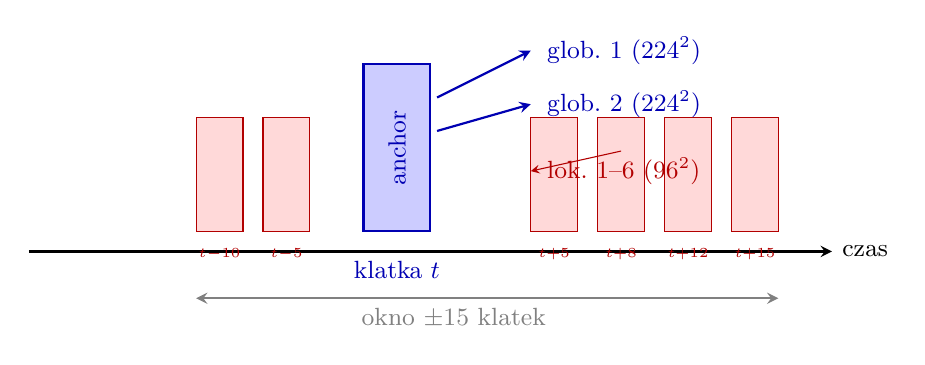
\begin{tikzpicture}[>=stealth, scale=0.85]
  % Oś czasu
  \draw[->, thick] (0,0) -- (12,0) node[right] {\small czas};

  % Klatka anchor
  \fill[blue!20] (5.0, 0.3) rectangle (6.0, 2.8);
  \draw[blue!70!black, thick] (5.0, 0.3) rectangle (6.0, 2.8);
  \node[blue!70!black, rotate=90] at (5.5, 1.55) {\small anchor};
  \node[below, blue!70!black] at (5.5, 0.0) {\small klatka $t$};

  % Widoki globalne z anchora
  \draw[->, blue!70!black, thick] (6.1, 2.3) -- (7.5, 3.0);
  \draw[->, blue!70!black, thick] (6.1, 1.8) -- (7.5, 2.2);
  \node[blue!70!black, anchor=west] at (7.6, 3.0) {\small glob.\ 1 ($224^2$)};
  \node[blue!70!black, anchor=west] at (7.6, 2.2) {\small glob.\ 2 ($224^2$)};

  % Klatki sąsiednie
  \foreach \x/\lab in {2.5/$t{-}10$, 3.5/$t{-}5$, 7.5/$t{+}5$, 8.5/$t{+}8$, 9.5/$t{+}12$, 10.5/$t{+}15$} {
    \fill[red!15] (\x, 0.3) rectangle ({\x+0.7}, 2.0);
    \draw[red!70!black] (\x, 0.3) rectangle ({\x+0.7}, 2.0);
    \node[below, red!70!black, font=\tiny] at ({\x+0.35}, 0.2) {\lab};
  }

  % Strzałki od sąsiadów do lokalnych widoków
  \node[red!70!black, anchor=west] at (7.6, 1.2) {\small lok.\ 1--6 ($96^2$)};
  \draw[->, red!70!black] (8.85, 1.5) -- (7.5, 1.2);

  % Okno ±15
  \draw[<->, gray, thick] (2.5, -0.7) -- (10.5+0.7, -0.7);
  \node[gray, below] at (6.35, -0.7) {\small okno $\pm 15$ klatek};
\end{tikzpicture}
\end{center}

\begin{itemize}[leftmargin=2em]
  \item \textbf{Widoki globalne} ($V_g = 2$): duże kadrowania z~\textbf{klatki anchor}
        (jeden konkretny moment $t$) --- te same piksele, różne wycinki.
  \item \textbf{Widoki lokalne} ($V_l = 6$): małe kadrowania z~\textbf{sąsiednich klatek}
        w~oknie $\pm 15$ klatek wokół anchora
        (np.\ klatka z~$t - 5$, $t + 8$, $t + 12$, \ldots).
\end{itemize}

\textbf{Dlaczego to działa?}
W~filmie chirurgicznym klatki oddalone o~kilka--kilkanaście klatek
pokazują \textbf{tę samą scenę}: to samo narzędzie, ta sama tkanka,
lekko zmieniony kąt.
Sieć uczy się: ``klatka z~sekundy 5.0 i~klatka z~sekundy 5.3
przedstawiają ten sam etap operacji $\Rightarrow$ bliskie embeddingi.''

\medskip
\textbf{Przewaga nad obrazami}: w~wideo nie potrzebujemy sztucznych augmentacji
(obroty, zmiana kolorów), bo \textbf{sam upływ czasu} naturalnie generuje
różne widoki tej samej sceny --- zmienia się oświetlenie,
kąt mikroskopu, pozycja narzędzia.
To są \textbf{prawdziwe} transformacje, nie syntetyczne.
\end{tcolorbox}

\subsection{Czytanie wzoru (\ref{eq:pred_loss}) --- loss predykcyjny}

\begin{tcolorbox}[colback=orange!5, colframe=orange!70!black, breakable,
  title={\textbf{Wzór (\ref{eq:pred_loss}) --- co dokładnie liczy $\mathcal{L}_{\text{pred}}$}}]

\[
\mathcal{L}_{\text{pred}} = \frac{1}{V}\sum_{v'=1}^{V}
\left\|\boldsymbol{\mu}_n - \mathbf{z}_{n,v'}\right\|_2^2,
\qquad
\boldsymbol{\mu}_n \triangleq \frac{1}{V_g}\sum_{v=1}^{V_g} \mathbf{z}_{n,v}
\]

\textbf{Krok 1 --- oblicz centroid $\boldsymbol{\mu}_n$:}

Bierzemy tylko widoki \textbf{globalne} (duże kadrowania) i~liczymy ich średnią:
\[
\boldsymbol{\mu}_n = \frac{\mathbf{z}_{n,1} + \mathbf{z}_{n,2}}{2}
\quad\text{(bo $V_g = 2$)}
\]

Centroid to ``punkt środkowy'' --- najlepsza reprezentacja tego, co sieć ``myśli''
o~obrazie $n$ na podstawie globalnych widoków.

\textbf{Dlaczego tylko globalne?}
Globalne widoki widzą duży fragment obrazu $\Rightarrow$ mają najwięcej informacji
$\Rightarrow$ są najbardziej wiarygodnym punktem odniesienia.

\bigskip
\textbf{Krok 2 --- zmierz odległość każdego widoku od centroidu:}

Dla \textit{każdego} widoku $v'$ (globalnego i~lokalnego) liczymy:
\[
\left\|\boldsymbol{\mu}_n - \mathbf{z}_{n,v'}\right\|_2^2
= \sum_{i=1}^{d} \left(\mu_{n,i} - z_{n,v',i}\right)^2
\]

To jest zwykły \textbf{kwadrat odległości euklidesowej} w~$\mathbb{R}^d$
--- suma kwadratów różnic po każdej współrzędnej.

\bigskip
\textbf{Krok 3 --- uśrednij:}

$\frac{1}{V}\sum_{v'=1}^{V}$ --- średnia z~$V$ odległości.

\medskip
\textbf{Co to wymusza?}
Jeśli ten sam kot sfotografowany z~bliska i~z~daleka daje
\textit{bliskie} embeddingi (mała odległość od centroidu),
to sieć nauczyła się rozpoznawać ``kotowość'' niezależnie od kadrowania.
\end{tcolorbox}

\subsection{Konkretny przykład liczbowy}

Weźmy $B = 2$ obrazy, $V_g = 2$ widoki globalne, $V_l = 1$ widok lokalny
($V = 3$), $d = 2$ wymiary (zamiast 128, dla prostoty), $\lambda = 0.05$.

\medskip
\textbf{Embeddingi} (sieć wypluwa):
\[
\begin{array}{c|ccc}
 & v=1 \text{ (glob.)} & v=2 \text{ (glob.)} & v=3 \text{ (lok.)} \\
\hline
\text{obraz } n=1 & \mathbf{z}_{1,1} = (1.0,\; 0.5) & \mathbf{z}_{1,2} = (0.8,\; 0.7)
  & \mathbf{z}_{1,3} = (1.3,\; 0.3) \\
\text{obraz } n=2 & \mathbf{z}_{2,1} = (-0.6,\; 1.2) & \mathbf{z}_{2,2} = (-0.4,\; 0.8)
  & \mathbf{z}_{2,3} = (-0.8,\; 1.0)
\end{array}
\]

\textbf{Część B --- predykcja (czytamy wierszami):}

Centroidy z~widoków globalnych:
\begin{align*}
\boldsymbol{\mu}_1 &= \tfrac{1}{2}\bigl((1.0, 0.5) + (0.8, 0.7)\bigr) = (0.9,\; 0.6) \\
\boldsymbol{\mu}_2 &= \tfrac{1}{2}\bigl((-0.6, 1.2) + (-0.4, 0.8)\bigr) = (-0.5,\; 1.0)
\end{align*}

Odległości od centroidu (obraz 1):
\begin{align*}
\|\boldsymbol{\mu}_1 - \mathbf{z}_{1,1}\|^2 &= (0.9-1.0)^2 + (0.6-0.5)^2 = 0.01 + 0.01 = 0.02 \\
\|\boldsymbol{\mu}_1 - \mathbf{z}_{1,2}\|^2 &= (0.9-0.8)^2 + (0.6-0.7)^2 = 0.01 + 0.01 = 0.02 \\
\|\boldsymbol{\mu}_1 - \mathbf{z}_{1,3}\|^2 &= (0.9-1.3)^2 + (0.6-0.3)^2 = 0.16 + 0.09 = 0.25
\end{align*}
\[
\mathcal{L}_{\text{pred}}^{(1)} = \frac{0.02 + 0.02 + 0.25}{3} = 0.097
\]

Analogicznie dla obrazu 2: powiedzmy $\mathcal{L}_{\text{pred}}^{(2)} = 0.063$.

\[
\text{Część B} = \frac{1 - 0.05}{2}(0.097 + 0.063) = \frac{0.95}{2} \cdot 0.16 = 0.076
\]

\textbf{Część A --- regularyzacja (czytamy kolumnami):}

Dla widoku $v = 1$: zbieramy $\{\mathbf{z}_{1,1}, \mathbf{z}_{2,1}\} = \{(1.0, 0.5),\; (-0.6, 1.2)\}$
i~sprawdzamy SIGRegiem, czy to $\mathcal{N}(\mathbf{0}, \mathbf{I})$.
Powiedzmy $\mathrm{SIGReg}_1 = 0.31$.
Analogicznie dla $v = 2, 3$.

\[
\text{Część A} = \frac{0.05}{3}(0.31 + 0.28 + 0.45) = \frac{0.05}{3} \cdot 1.04 = 0.017
\]

\textbf{Pełny loss:}
\[
\mathcal{L}_{\text{LeJEPA}} = \underbrace{0.017}_{\text{SIGReg}} + \underbrace{0.076}_{\text{predykcja}} = 0.093
\]

\begin{keyinsight}[Dwa cele, jedna liczba]
Widzimy, że predykcja dominuje ($0.076$ vs $0.017$) --- tak ma być przy $\lambda = 0.05$.
Sieć skupia się na \textbf{semantycznej spójności} widoków (``ten sam kot $\Rightarrow$ bliskie wektory''),
a~SIGReg działa w~tle jako \textbf{strażnik} (``ale nie kolapsuj do jednego punktu --- rozpychaj się gaussowsko!'').
\end{keyinsight}

\subsection{Podsumowanie: regularyzacja vs predykcja}

\begin{center}
\renewcommand{\arraystretch}{1.3}
\begin{tabular}{lcc}
\toprule
& \textbf{Regularyzacja (SIGReg)} & \textbf{Predykcja} \\
\midrule
\textbf{Iteruje po} & widokach ($v$) & obrazach ($n$) \\
\textbf{Zbiera} & embeddingi jednego widoku z~$B$ obrazów & embeddingi jednego obrazu z~$V$ widoków \\
\textbf{Sprawdza} & ``czy rozkład $\approx \mathcal{N}(\mathbf{0}, \mathbf{I})$?'' & ``czy widoki się zgadzają?'' \\
\textbf{Chroni przed} & kolapsem (wszystko $\to$ jeden punkt) & chaosem (losowe embeddingi) \\
\textbf{Waga} & $\lambda = 0.05$ (5\%) & $1 - \lambda = 0.95$ (95\%) \\
\bottomrule
\end{tabular}
\end{center}

